\documentclass[b5paper,final]{article}
% Add "final" option in the article to remove todo
\usepackage[tight,common_math_textnormal,todonotes,math_base_note,math_simple]{gatmeo}
\usepackage{tikz-cd}
\newcommand{\mynewpage}{\newpage}

\title{\bf{
Hypertoric Varieties Arose from Graphs
}}

\newcommand{\ansonlaw}{\FirstBigRestSmallCaps{Sum kiu Law}\thanks{sklaw@math.cuhk.edu.hk}}
\renewcommand{\omegat}{\FirstBigRestSmallCaps{Nok to Omega Tong}\thanks{onttong@math.cuhk.edu.hk}}

\author{\ansonlaw\ {\small{AND}} \omegat\\\\
\emph{Department of Mathematics, The Chinese University of Hong Kong, Hong Kong}
}
\date{}
%sklaw@math.cuhk.edu.hk, onttong@math.cuhk.edu.hk\\\\

\newcommand{\noskipline}{\vspace{-1.5em}}

\renewcommand{\epsilon}{\varepsilon}
\renewcommand{\phi}{\varphi}
\newcommand{\NN}{\mathbb{N}}
\newcommand{\ZZ}{\mathbb{Z}}
\tikzcdset{
    cells={font=\everymath\expandafter{\the\everymath\displaystyle}},
}

% Hypertoric Variety
\newcommand{\MM}{\mathcal{M}}
\newcommandx*\Mper[1][1=\Gamma]{\mathcal{M}^{\mathrm{per}}(#1)}
\newcommandx*\Mperchar[2][2=\Gamma]{\mathcal{M}^{\mathrm{per}}_{#1}(#2)}
\newcommandx*\Hper[1][1=\Gamma]{\mathcal{A}^{\mathrm{per}}(#1)}
\newcommandx*\Hperchar[2][2=\Gamma]{\mathcal{A}^{\mathrm{per}}_{#1}(#2)}
\newcommandx*\Rper[2][1=\bullet, 2=\Gamma]{\mathcal{R}_{\mathrm{per}}^{#1}(#2)}
\newcommandx*\SRper[2][1=\bullet, 2=\Gamma]{\mathcal{SR}_{\mathrm{per}}^{#1}(#2)}
\newcommandx*\Mfin[1][1=\Gamma]{\mathcal{M}(#1)}
\newcommandx*\Mfinchar[2][2=\Gamma]{\mathcal{M}_{#1}(#2)}
\newcommandx*\Hfinchar[2][2=\Gamma]{\mathcal{A}_{#1}(#2)}
\newcommandx*\Hfin[1][1=\Gamma]{\mathcal{A}(#1)}
\newcommandx*\Rfin[2][1=\bullet, 2=\Gamma]{\mathcal{R}^{#1}(#2)}
\newcommandx*\SR[2][1=\bullet, 2=\Gamma]{\mathcal{SR}^{#1}(#2)}
\newcommandx*\Mmul[1][1=\Gamma]{\mathcal{M}^{\mathrm{mul}}(#1)}
\newcommandx*\idealIper[1][1=\Gamma]{I_{\mathrm{per}}(#1)}
\newcommandx*\idealI[1][1=\Gamma]{I(#1)}
\newcommand{\opendisc}{\mathbb{D}}
\newcommandx*\Betti[1][1=\Gamma]{\mathfrak{B}(#1)}
\newcommandx*\Dolbeault[1][1=\Gamma]{\mathfrak{D}(#1)}

% Core and Toric
\newcommandx*\corefin[1][1=\Gamma]{\mathcal{L}(#1)}
\newcommandx*\coreper[1][1=\Gamma]{\mathcal{L}^{\mathrm{per}}(#1)}
\newcommandx*\toricP[1][1=P]{\mathcal{X}(#1)}
\newcommandx*\fixptP[1][1=B]{P_{#1}}
\newcommandx*\toricB[1][1=B]{\mathcal{X}(#1)}

% Complex
% Group Cohomology Complex
\newcommand{\pGC}{\mathfrak{C}} 
\newcommandx*\GC[3][1=\bullet,2=\bullet,3=\Gamma]{\mathfrak{C}^{#1,#2}(#3)} % Our complex: Group Cohomology
\newcommand{\dGC}{\delta} % Our complex: Group Cohomology
\newcommand{\dGCbar}{\bar{\delta}} % Our complex: Group Cohomology
\newcommand{\fGC}{\phi}
\newcommand{\gGC}{\psi}
\newcommand{\hGC}{\eta}
%--- Group Cohomology Complex with e
\newcommandx*\GCe[4][1=\bullet,2=\bullet,3=\Gamma,4=e]{\mathfrak{C}^{#1,#2}(#3,#4)}
\newcommand{\dGCe}{\delta_e}
\newcommand{\fGCe}{\mathfrak{f}}
\newcommand{\gGCe}{\mathfrak{g}}
\newcommand{\hGCe}{\mathfrak{h}}
%--- CKS
\newcommandx*\GCS[2][1=\bullet,2={\Gamma, S}]{\mathfrak{D}^{#1}(#2)}
\newcommandx*\dGCS[1][1=S]{\dGC_{#1}}
\newcommandx*\fGCS[1][1=S]{\fGC_{#1}}
\newcommandx*\gGCS[1][1=S]{\gGC_{#1}}
\newcommandx*\hGCS[1][1=S]{\hGC_{#1}}
\newcommandx*\CKS[4][1=\bullet,2=\bullet,3=\bullet,4=\Gamma]{\mathfrak{C}^{#1,#2,#3}(#4)} % CKS
\newcommandx*\grCKS[4][1=\bullet,2=\bullet,3=\bullet,4=\Gamma]{I^{#1, #2}\mathfrak{C}^{#3}(#4)} % CKS
\newcommandx*\CKSdiffgrading[3][1=\bullet,2=\bullet,3=\Gamma]{\mathfrak{C}'^{#1,#2}(#3)} % CKS
\newcommand{\dCKS}{d} %CKS Complex
\newcommand{\fCKS}{f}
\newcommand{\gCKS}{g}
\newcommand{\hCKS}{h}
\newcommandx*\HT[3][1=\bullet,2=\bullet,3=\Gamma]{\mathfrak{K}_{\mathrm{per}}^{#1, #2}(#3)}
\newcommandx*\grHT[3][1=\bullet,2=\bullet,3=\Gamma]{I^{#1}\mathfrak{K}_{\mathrm{per}}^{#2}(#3)}
\newcommand{\dHT}{\dCKS_{\mathrm{per}}}
\newcommandx*\HTalt[2][1=\bullet,2=\Gamma]{\tilde{\mathfrak{K}}^{#1}(#2)}
\newcommand{\dHTalt}{\tilde{\dCKS}_{\mathrm{per}}}
\newcommand{\fHT}{\fCKS_{\mathrm{per}}}
\newcommand{\gHT}{\gCKS_{\mathrm{per}}}
\newcommand{\hHT}{\hCKS_{\mathrm{per}}}
\newcommandx*\HTfin[3][1=\bullet,2=\bullet,3=\Gamma]{\mathfrak{K}^{#1, #2}(#3)}
\newcommandx*\grHTfin[3][1=\bullet,2=\bullet,3=\Gamma]{I^{#1}\mathfrak{K}^{#2}(#3)}
\newcommand{\dHTfin}{\dCKS}
\newcommand{\fHTfin}{\fCKS}
\newcommand{\gHTfin}{\gCKS}
\newcommand{\hHTfin}{\hCKS}
\newcommandx*\CPX[3][1=\bullet,2=\bullet,3=\Gamma]{\mathfrak{D}^{#1,#2}(#3)} % Intermediate complex
\newcommandx*\euler[3][3=\Gamma]{\eta^{#1, #2}(#3)}

% Graph and Matroids
\newcommandx*\Tutte[2][1=\Gamma]{T(#1;\, #2)}
\newcommandx*\hpoly[2][1=\Gamma]{h(#1;\, #2)}
\newcommandx*\HTutte[2][1=\Gamma]{H(#1;\, #2)}
\newcommandx*\seqn[1][1=n]{[-#1,#1]}
\newcommand{\loopgraph}{{\bigcirc\!\!\bullet}}
\newcommand{\bridgegraph}{{\bullet\mspace{-7mu}-\mspace{-7mu}\bullet}}
\newcommand{\supnorm}[1]{\| #1 \|_{\infty}} 

\newcommand{\del}{\setminus}
\newcommand{\con}{\mathbin{/}}
\newcommand{\Gammaper}{\Gamma_{\mathrm{per}}}
\newcommandx*\tree[2][2=\Gamma]{\mathcal{T}_{#2}(#1)}
\newcommandx*\treefunction[1][1=\Gamma]{\mathcal{T}_{#1}}
\newcommandx*\cotreefunction[1][1=\Gamma]{\mathcal{T}_{#1}^*}
\newcommandx*\cotree[2][2=\Gamma]{\mathcal{T}_{#2}^*(#1)}
\newcommandx*\face[2][1=\bullet,2=\Gamma]{F_{#1}(#2)}
\newcommandx*\faceshelling[3][2=\bullet,3=\Gamma]{F_{#2}^{(#1)}(#3)}
\newcommandx*\faceper[2][1=\bullet,2=\Gamma]{F^{\mathrm{per}}_{#1}(#2)}
\newcommandx*\pair[3][3=\Gamma]{\langle #1, #2 \rangle_{#3}}
\newcommandx*\cotreein[2][2=\Gamma]{\mathcal{D}_{#2}(#1)}
\newcommandx*\cotreeinper[2][2=\Gamma]{\mathcal{D}^\per_{#2}(#1)}
\newcommandx*\cotreeinfunction[1][1=\Gamma]{\mathcal{D}_{#1}}
\newcommandx*\externalactivity[2][2=\Gamma]{EA_{#2}(#1)}
\newcommandx*\internalactivity[2][2=\Gamma]{IA_{#2}(#1)}
\newcommand{\intp}[1]{\iota_{#1}} % interior product
\newcommandx*\fundcycle[2][2=\Gamma]{C_{#2}(#1)}
\newcommandx*\fundcyclewithtree[3][2=\Gamma,3=T]{C_{#2}(#3,#1)}
\newcommandx*\basis[2][1=\bullet,2=\Gamma]{\mathcal{B}_{#1}(#2)}
\newcommandx*\basisper[2][1=\bullet,2=\Gamma]{\mathcal{B}^\per_{#1}(#2)}

\newcommandx*\SE[3][1=,3=]{
  \ifstrempty{#3}
  {\ifstrempty{#1}{E^\bullet_{#2}}{#1_{#2}}}
  {\ifstrempty{#1}{E_{#2}(#3)}{#1_{#2}}}
}
\newcommandx*\HMGZ[2][1=\Gamma,2=\bullet]{H^{#2}(\MM(#1),\mathbb{Z})}
\newcommand{\hCCC}{\hat{\mathfrak{C}}}

\newcommand{\per}{\mathrm{per}}

% Math Operations
\newcommand{\HH}{\mathrm{H}}
\newcommandx*\Ext[1][1=\bullet]{\bigwedge\nolimits^{#1}}
\newcommandx*\Sym[1][1=\bullet]{\mathrm{Sym}^{#1}}
\newcommand{\sgn}{\mathrm{sgn}}
\newcommand{\coker}{\operatorname{coker}}
\renewcommand{\im}{\operatorname{Im}}
\newcommand{\supp}{\mathrm{supp}}
\newcommand{\Hom}{\mathrm{Hom}}

% Group Cohomology
\newcommand{\invar}[1]{\Gamma_{#1}}
\newcommandx*\Rder[1][1=\bullet]{R^{#1}}
\newcommandx*\totRder[1][1=\bullet]{\mathbb{R}^{#1}}

% Homotopy Equivalence
\newcommand{\choice}[1]{[#1]} % choice for HTfin equiv
\newcommandx*\intord[2][2=S]{[#2]^{#1}} % integration order for GCS equiv
\newcommandx*\hyppl[2][2=S]{\alpha^{#2}_{#1}} % hyperplane for GCS equiv

\makeatletter
\newcommand{\GIT}[1][\@nil]{%
  \def\tmp{#1}%
  \ifx\tmp\@nnil
    /\!\!/%
  \else
    /\!\!/_{\! #1}%
  \fi
}
\newcommand{\HQ}[1][\@nil]{%
  \def\tmp{#1}%
  \ifx\tmp\@nnil
    /\!\!/\!\!/\!\!/%
  \else
    /\!\!/\!\!/\!\!/_{\! #1}%
  \fi
}
\makeatother

\newcommand{\Diff}{\mathrm{Diff}}
\newcommand{\Sympl}{\mathrm{Sympl}}
\newcommand{\acton}{\curvearrowright}
\newcommand{\smth}{C^\infty}
\newcommand{\df}{\Omega}
\newcommand{\vf}{\mathrm{Vec}}
\newcommand{\svf}{\mathrm{Vec}_\mathrm{sym}}
\newcommand{\hvf}{\mathrm{Vec}_\mathrm{ham}}
\newcommand{\ind}[1]{#1^\#}
\newcommand{\lied}[1]{\mathcal{L}_{#1}}
\newcommand{\intd}[1]{\iota_{#1}}

\begin{document}
\maketitle
\vspace{-3.5em}
%\input{abstract}

\thispagestyle{empty}
\tableofcontents
\listoftodos

\newpage
\section{Combinatorics of Graphs}
\section{Hypertoric Varieties}
\subsection{GIT}
\subsection{Stability Condition}
For both $\theta$ and $\lambda$
\section{GKM Graph of Hypertoric}
\subsection{Fix Points}
\subsection{Connecting P1}
How $\theta$ effects the splitting of $S^+$
\subsection{Matroid Polytope}
\subsection{Equivariant Cohomology of Hypertoric}
\section{Line Bundles on Hypertoric}
\section{Steinberg Correspondences}
\subsection{Primitive Coroots and Hyperplane}
\subsection{Steinberg Varieties}

\section{Comparing Stability Condition with Quiver Varieties}

\appendix
\section{Symplectic Reduction for Toric Varieties}

\subsection{Symplectic and Hamiltonian Action}

It is natural to consider the subclass of Lie group actions on symplectic manifolds that act by symplectomorphisms. Turns out, there is a smaller class of actions, called the Hamiltonian actions, that are of interest.

\begin{definition}{Symplectic Action}
    Lie group action $\rho : G \to \Diff(M)$ if $\im(\rho) \subseteq \Sympl(M)$.
\end{definition}

\begin{proposition}{}
    If $G \acton M$ is symplectic, then $\ind{X} \in \svf(M)$ for all $X \in \mathfrak{g}$.
    \inquiry{Converse?}
\end{proposition}

\begin{definition}{Hamiltonian Action}
    $G \acton M$ symplectic with a \vocab{moment map} $\mu : M \to \mathfrak{g}^*$ such that
    \begin{enumerate}
        \item $\mu$ is $G$-equivariant wrt $G \acton M$ and $G \acton \mathfrak{g}^*$ by the coadjoint action (see Definition~\ref{def:coadj}), and
        \item for all $X \in \mathfrak{g}$, considered as $X : \mathfrak{g}^* \to \mathbb{R}$, $d(X \circ \mu) = \intd{\ind{X}}\omega$.
    \end{enumerate}
\end{definition}

\inquiry{Hamiltonian action implies induced vector fields are Hamiltonian? Converse?}

\begin{lemma}{}
    Let $\mu : M \to \mathfrak{g}^*$ be a moment map and suppose $G$ is abelian. Then, $\mu + \alpha$ is also a moment map for all $\alpha \in \mathfrak{g}^*$.
    \begin{proof}
        This is because the coadjoint action for abelian Lie group is trivial.
    \end{proof}
\end{lemma}

\begin{proposition}[prop:cot moment]{Moment Map on Cotangent Bundle}
    Let $M$ be a smooth manifold with a $G$ action. Then, there is a canonical choice of the moment map $\mu : T^*M \to \mathfrak{g}^*$ of the induced $G$-action on the symplectic manifold $T^*M$.
    \begin{proof}
        Let $\pi : T^*M \to M$ be the projection. Recall from Proposition~\ref{prop:cot sympl} that we have the tautological form $\theta$ and the symplectic form $\omega$ on $T^*M$. We claim that the induced action $G \acton T^*M$, defined by $g \cdot (p, \alpha) = (g \cdot p, d(g^{-1})_p^*(\alpha))$, is Hamiltonian and has a canonical choice of moment map $\mu : T^*M \to \mathfrak{g}^*$.
        
        Let $X \in \mathfrak{g}$. Denote the induced vector field of $X$ on $M$ by $\ind{X}$, and on $T^*M$ by $\ind{\tilde{X}}$ temporarily. By Lemma~\ref{lem:prop_of_DLI},
        \begin{equation*}
            \intd{\ind{\tilde{X}}}\omega = \intd{\ind{\tilde{X}}} (-d\theta) = d(\intd{\ind{\tilde{X}}}\theta) + \lied{\ind{\tilde{X}}}\theta = d(\theta(\ind{\tilde{X}})) + \lied{\ind{\tilde{X}}}\theta.
        \end{equation*}
        We claim that $\lied{\ind{\tilde{X}}}\theta=0$. For the sake of readability, let us denote the diffeomorphisms $p \mapsto \exp(tX) \cdot p$ and $(p, \alpha) \mapsto \exp(tX) \cdot (p, \alpha)$ by $\varphi$ and $\tilde{\varphi}$ respectively. Then,
        \begin{align*}
            \lied{\ind{\tilde{X}}}\theta_{(p, \alpha)} &= \frac{d}{dt} \left[\tilde{\varphi}^*\theta_{(p, \alpha)}\right]_{t=0} = \frac{d}{dt} \left[d\tilde{\varphi}_{(p, \alpha)}^*(\theta_{\tilde{\varphi}(p, \alpha)})\right]_{t=0} = \frac{d}{dt} \left[d\tilde{\varphi}_{(p, \alpha)}^*(d\pi_{\tilde{\varphi}(p, \alpha)}^*(d(\varphi^{-1})_p^*(\alpha)))\right]_{t=0} \\
            &= \frac{d}{dt} \left[d(\varphi^{-1} \circ \pi \circ \tilde{\varphi})_{(p, \alpha)}^*(\alpha)\right]_{t=0} = \frac{d}{dt} \left[d(\varphi^{-1} \circ \varphi \circ \pi)_{(p, \alpha)}^*(\alpha)\right]_{t=0} = \frac{d}{dt} \left[d\pi_{(p, \alpha)}^*(\alpha)\right]_{t=0} \\
            &= 0.
        \end{align*}
        The result is 0 since the expression in the differentiation sign does not depend on $t$ anymore. Thus, we have $\intd{\ind{\tilde{X}}}\omega = d(\theta(\ind{\tilde{X}}))$. The moment map requires $d(X \circ \mu) = \intd{\ind{\tilde{X}}}\omega$, hence a natural choice would be to define $X \circ \mu = \theta(\ind{\tilde{X}})$. To expand further, note that for all $(p, \alpha) \in T^*M$,
        \begin{align*}
            \theta(\ind{\tilde{X}})(p, \alpha) &= \theta_{(p, \alpha)}(\ind{X}_{(p, \alpha)}) = \alpha(d\pi_{(p, \alpha)}(\ind{X}_{(p, \alpha)})) = \alpha \left( d\pi_{(p, \alpha)} \left( \frac{d}{dt} [\exp(tX) \cdot (p, \alpha)]_{t=0} \right) \right) \\
            &= \alpha \left( \frac{d}{dt} [\pi(\exp(tX) \cdot (p, \alpha))]_{t=0} \right) = \alpha \left( \frac{d}{dt} [\exp(tX) \cdot p]_{t=0} \right) = \alpha(\ind{X}_p).
        \end{align*}
        Hence, the moment map is described by $\mu(p, \alpha)(X) = \alpha(\ind{X}_p)$ for all $(p, \alpha) \in T^*M$ and $X \in \mathfrak{g}$.
    \end{proof}
\end{proposition}

\subsubsection*{Example Calculation of Moment Map}

\begin{example}[exp:Cn_moment]{$\mathbb{T}^n \acton \mathbb{C}^n$}
    In Example~\ref{exp:Cn_ind_vf}, we computed that $\ind{X_i} = -2\pi y_i \frac{\partial}{\partial x_i} + 2\pi x_i \frac{\partial}{\partial y_i}$. Then,
    \begin{align*}
        \intd{\ind{X_i}}\omega &= \biggl(\sum_j dx_j \wedge dy_j\biggr)\left(-2\pi y_i \frac{\partial}{\partial x_i} + 2\pi x_i \frac{\partial}{\partial y_i}\right) = dx_i \left(-2\pi y_i \frac{\partial}{\partial x_i}\right) \, dy_i - dy_i\left(2\pi x_i \frac{\partial}{\partial y_i}\right) \, dx_i \\
        &= -2\pi (x_i \, dx_i + y_i \, dy_i).
    \end{align*}
    Thus, $\intd{\ind{X_i}}\omega = d(-\pi(x_i^2 + y_i^2)) = d(-\pi|z_i|^2)$. Note that $X_i : (\mathfrak{t}^n)^* \to \mathbb{R}$ is regarded as the $i$th coordinate map. It follows that $\mu(z_1, \dots, z_n) = (-\pi|z_1|^2, \dots, -\pi|z_n|^2)$ is a choice of moment map.
\end{example}

\subsection{Symplectic Reduction}

The goal here is to define a suitable quotient of a symplectic manifold by a Hamiltonian action. However, the naive quotient does not have nice properties in general. Thus, we need to apply the method of symplectic reduction.

Assume we have a Hamiltonian action $G \acton M$ with moment map $\mu : M \to \mathfrak{g}$, where $G$ is compact.

\begin{lemma}{}
    $\mu^{-1}(0) \subseteq M$ is $G$-invariant.
    \begin{proof}
        Let $g \in G$ and $p \in \mu^{-1}(0)$. Then, $\mu(g \cdot p) = \mathrm{Ad}_g^*(\mu(p)) = \mathrm{Ad}_g^*(0) = 0$. Thus, $g \cdot p \in \mu^{-1}(0)$.
    \end{proof}
\end{lemma}

\begin{definition}{Symplectic Reduction}
    $M \GIT G = \mu^{-1}(0)/G$, assuming the restricted action $G \acton \mu^{-1}(0)$ is free.
    \begin{remark}
    When $G$ is abelian, we can reduce at other levels, i.e. replace $\mu^{-1}(0)$ by $\mu^{-1}(\xi)$ for other $\xi \in \mathfrak{g}^*$.
        This is because abelian $\implies$ conjugation is trivial $\implies$ coadjoint action is trivial $\implies$ $\mu^{-1}(\xi)$ is $G$-invariant for all $\xi \in \mathfrak{g}^*$.
    \end{remark}
\end{definition}

\begin{theorem}{Marsden-Weinstein-Meyer Theorem}
    Assume that the restricted action $G \acton \mu^{-1}(0)$ is free. Then,
    \begin{enumerate}
        \item $M \GIT G$ is a smooth manifold and $\mu^{-1}(0) \to M \GIT G$ is a principal bundle, and
        \item there is a symplectic form $\omega_{\mathrm{red}}$ on $M \GIT G$ satisfying $\iota^*\omega = \pi^*\omega_{\mathrm{red}}$.
    \end{enumerate}
    \begin{equation}
        \begin{tikzcd}
            \mu^{-1}(0) \arrow[r, hook, "\iota"] \arrow[d, two heads, "\pi"'] & M \\
            M \GIT G & {}
        \end{tikzcd}
    \end{equation}
    \begin{proof}
        Proof of (a) follows from Theorem~\ref{thm:QMT}. Proof of (b) is omitted.
    \end{proof}
\end{theorem}

\subsubsection*{Symplectic Reduction of a Free and Proper Action on Cotangent Bundle}

Following Proposition~\ref{prop:cot sympl} and Proposition~\ref{prop:cot moment}, we give a general calculation for the symplectic reduction of the cotangent bundle. This will also show the motivation for using symplectic reduction as a quotient.

\begin{proposition}[prop:cot red]{}
    Let $M$ be a smooth manifold with a free and proper $G$-action. This induces a Hamiltonian $G$-action on $T^*M$ with moment map $\mu : T^*M \to \mathfrak{g}^*$. Then, $(T^*M) \GIT G \cong T^*(M/G)$.
    \begin{proof}
        As $G \acton M$ is free and proper, by Theorem~\ref{thm:QMT}, we know that $M/G$ is a smooth manifold. Let $\pi : T^*M \to M$ be the projection and consider the induced action $G \acton T^*M$. We already defined the symplectic form $\omega$ on $T^*M$ and the moment map $\mu : T^*M \to \mathfrak{g}^*$. We claim that $(T^*M) \GIT G \cong T^*(M/G)$ as vector bundles over $M/G$.
        
        Note that we have the following isomorphisms, where $\perp$ denotes the annihilator.
        \begin{align*}
            T_{[p]}(M/G) \cong T_pM / T_p(G \cdot p) && T_{[p]}^*(M/G) \cong T_p(G \cdot p)^\perp \subseteq T_p^*M
        \end{align*}
        Let $\pi : TM \to T(M/G)$ be the projection. Note that $\ker(\pi_p) \cong T_p(G \cdot p)$. Using the fact that $G \acton M$ is free, we can show that $\ker(\pi_p) = \{ v \in T_pM \mid \pi(p, v) = 0 \} = \{ \ind{X}_p \mid X \in \mathfrak{g} \} \cong \mathfrak{g}$ for all $p \in M$.
    
        Let $\tau : (T^*M) \GIT G \to M/G$ be the map induced by the $G$-equivariant map $\mu^{-1}(0) \to M$. Then, $\tau$ is surjective since for all $p \in M$, $(p, 0) \in \mu^{-1}(0)$. Let $p \in M$. Since $G \acton M$ is free, the fiber $\tau^{-1}([p])$ has the following description.
        \begin{align*}
            \tau^{-1}([p]) &= \{ [p, \alpha] \mid (p, \alpha) \in \mu^{-1}(0) \} \\
            &\cong \{ \alpha \in T_p^*M \mid \mu(p, \alpha) = 0 \} = \{ \alpha \in T_p^*M \mid \alpha(\ind{X}_p) = 0 \quad \forall X \in \mathfrak{g} \} \\
            &= \{ \ind{X}_p \mid X \in \mathfrak{g} \}^\perp = \ker(\pi_p)^\perp \cong T_p(G \cdot p)^\perp = T_p^*M
        \end{align*}
        This gives the required isomorphism $(T^*M) \GIT G \cong T^*(M/G)$.
        \end{proof}
\end{proposition}

\subsection{Symplectic Reduction from Physics POV}

A symplectic manifold is a natural object when studying physics.
We will not get into the details of it, but will give an overview of how does symplectic manifold arises.

According to Newton's Law, we can predict the future by knowing the position or velocity of every object in the world. Mathematically speaking, if we consider a point-like particle moving in space described by a smooth function $x:\mathbb{R}\rightarrow \mathbb{R}^3$, such a function satisfies the differential equation:
\[
  m\frac{d^2}{dt^2}x=F(x,\frac{d}{dt}x,t)
\]
for some function $F$. Physicists then study what is the trajectory of the particle for different $F$.

Given this, to describe a physical system we need to specify both position and velocity. The space that describes all the possible positions is the \vocab{configuration space}. The space that describes both positions and velocities is called \vocab{phase space}.

\begin{example}[exp:physics_realline]{}
  Consider an object moving in $\mathbb{R}^3$. Then the phase space is $\mathbb{R}^6$, with axes representing $x\in \mathbb{R}^3$ and $\frac{d}{dt}x$, the position and the velocity, or $T\mathbb{R}^3$.
\end{example}

In general, given the configuration space as $X$, the phase space will be $TX$.
However, instead of considering the velocity, we may consider the dual concept of, momentum. There is a canonical conversion between the velocity and a so-called \vocab{generalized momenta}, which we will not describe here. After such identification, the phase space (position and momentum) can then be identified with $T^*X$ which by \Cref{prop:cot sympl} is a symplectic manifold.

Yet, there may be many symmetries that lie in a physical problem. Consider \Cref{exp:physics_realline}, and imagine the particle is under the potential energy of gravitational force. The horizontal position of the particle at the start of the experiment does not affect the trajectory of it. Indeed, the experiment is invariant up to translation (allow us to be sloppy with the definition here). Hence to study the physical phenomenon, we may as well just quotient away this extra freedom. A mathematical statement of the physics problem will be: we want to study the phase space being quotient by a group acting on it. In the example we considered, the group $\mathbb{R}$ act (by translation) on the $T^*\mathbb{R}$. The method to study this quotient is to use symplectic reduction.

\subsubsection*{Symplectic Reduction in Action}

\begin{example}[exp:]{Translation}
  Consider the setting of \Cref{exp:physics_realline} where $G=\mathbb{R}^2$, $X=\mathbb{R}^{3}, M=T^*X$ with coordinate $q\in X$ and $p\in T^*$, whcih is symplectic with the canonical symplectic form. Define the action act to be
  \[
    v\cdot (q,p)=(q+(v_1,v_2,0),p), v\in G, (q,p)\in M,
  \]
  i.e. $v$ acts on $q$ on the first 2 coordinates. Since gravity only affects the $z$-axis direction, when considering the experiment of a particle moving along $\mathbb{R}^3$, it is natural to quotient out the $x,y$ direction. Mathematically, the moment map is then given by $\mu:\mathbb{R}^6n\rightarrow \mathbb{R}^2\simeq (T_e\mathbb{R}^3)^*|_{\mathbb{R}^2\times \SB{0}}$ given by projecting onto the first two momentum coordinate: $(q,p)\mapsto (p_1,p_2)$. And the symplectic reduction $\mu^{-1}(0)/\mathbb{R}^2=T^*\mathbb{R}$, which means to study the object free falling, we can just restrict ourselves to the one dimensional $z$-axis.
\end{example}
%
%\begin{example}[exp:]{Rigid Body}
%  We will study the example of a rigid body: A rigid body is defined to be a configuration of point-like bodies $x_i$ in $\mathbb{R}^3$ with the system of constraints of the form $|x_i-x_j|=C_{ij}$. It is easy to see that the configuration space of a rigid body is diffeomorphic to $X=SO(3)\times \mathbb{R}^3$. Consider the symplectic reduction of $T^*X$ by $\mathbb{R}^3\times SO(3)$. $T^*X//\mathbb{R}^3$ by the previous example is $T^*SO(3)$.
%\end{example}

\subsection{Symplectic Toric Manifold}

We are now restricted to studying a nice class of Hamiltonian torus action. Our goal is to classify them using a kind of polytope, which arises as the image of the moment map.

\begin{definition}{Symplectic Toric Manifold}
    A compact connected $2n$-dimensional symplectic manifold $M$ with a effective (i.e. $T \to \Sympl(M)$ is injective) $n$-dimensional torus action $T \acton M$ that is Hamiltonian, i.e. with a moment map $\mu : M \to \mathfrak{t}^*$.
    \begin{remark}
        If we pick an isomorphism $T \cong \mathbb{T}^n$, then we have $\mathfrak{t} \cong \mathbb{R}^n$.
    \end{remark}
    \begin{remark}
        Note that $2n$-dimensional symplectic toric manifolds correspond to $n$-dimensional connected projective toric varieties.
        \inquiry{How precise is this correspondence?}
    \end{remark}
\end{definition}

\begin{definition}{Delzant Polytope}
    Convex polytope $\Delta \subseteq \mathbb{R}^d$ such that
    \begin{enumerate}
        \item it is simple, i.e. there are $d$ edges meeting at each vertex,
        \item it is rational, i.e. for all vertex $x$, each edge meeting at $x$ is of the form $x+tu, t \geq 0$ for some $v \in \mathbb{Z}^d$, and
        \item it is smooth, i.e. for all vertex $x$, there exist $v_1, \dots, v_n \in \mathbb{Z}^d$ that spans the $d$ edges such that $(v_1, \dots, v_d)$ forms a $\mathbb{Z}$-basis of $\mathbb{Z}^d$.
    \end{enumerate}
\end{definition}

\begin{lemma}[lem:vd_Delz]{}
    A Delzant polytope $\Delta \subseteq (\mathbb{R}^d)^*$ can be described by $a_1, \dots, a_n \in \mathbb{Z}^d$ and $r_1, \dots, r_n \in \mathbb{R}$, where $n$ is the number of facets of $\Delta$, such that
    \begin{equation*}
        \Delta = \{ x \in (\mathbb{R}^d)^* \mid \langle x, a_i \rangle \leq r_i \  \forall 1 \leq i \leq n \}.
    \end{equation*}
    Moreover, by the property of Delzant polytope, $(a_1, \dots, a_n)$ spans $\mathbb{Z}^d$.
\end{lemma}

\begin{theorem}{}
    For every symplectic toric manifold $(M, \omega, \mathbb{T}^d, \mu)$, $\im(\mu) \subseteq (\mathbb{R}^d)^*$ is a Delzant polytope. Conversely, any Delzant polytope $\Delta \subseteq (\mathbb{R}^d)^*$ gives a symplectic toric manifold. The above constructions are inverses of each other.
    \begin{remark}
        In particular, this theorem tells us that we can construct a symplectic toric manifold from a Delzant polytope. This construction resembles that of toric varieties.
    \end{remark}
    \begin{proof}
        Idea: Let $n$ be the number of facets of $\Delta$ and let $k=n-d$. Then, $\Delta$ defines a Hamiltonian action $\mathbb{T}^k \acton \mathbb{C}^n$. We then obtain the symplectic toric manifold by $M = \mathbb{C}^n \GIT \mathbb{T}^k$.
        
        Let $a_1, \dots, a_n \in \mathbb{R}^d$ and $r_1, \dots, r_n \in \mathbb{R}$ satisfying
        \begin{equation*}
            \Delta = \{ x \in (\mathbb{R}^d)^* \mid \langle x, a_i \rangle \leq r_i \  \forall 1 \leq i \leq n \}.
        \end{equation*}
        Consider the map $\pi : \mathbb{R}^n \to \mathbb{R}^d$ defined by $e_i \mapsto a_i$. By Lemma~\ref{lem:vd_Delz}, $\pi$ is surjective and maps $\mathbb{Z}^n$ onto $\mathbb{Z}^d$. Hence, there is an induced map $\mathbb{R}^n/\mathbb{Z}^n \cong \mathbb{T}^n \to \mathbb{R}^d/\mathbb{Z}^d \cong \mathbb{T}^d$. Let $\iota : \mathbb{T}^k \to \mathbb{T}^n$ be its kernel, where $k=n-d$. Explicitly, we have the following exact sequences.
        \begin{equation*}
            \begin{tikzcd}[row sep=small]
                1 \arrow[r] & \mathbb{T}^k \arrow[r, "\iota"] & \mathbb{T}^n \arrow[r, "\pi"] & \mathbb{T}^d \arrow[r] & 1 \\
                0 \arrow[r] & \mathfrak{t}^k \arrow[r, "\ind{\iota}"] & \mathfrak{t}^n \arrow[r, "\ind{\pi}"] & \mathfrak{t}^d \arrow[r] & 0 \\[-2ex]
                {} & {} & e_i \arrow[r, maps to] & v_i & {} \\
                0 \arrow[r] & (\mathfrak{t}^d)^* \arrow[r, "(\ind{\pi})^*"] & (\mathfrak{t}^n)^* \arrow[r, "(\ind{\iota})^*"] & (\mathfrak{t}^k)^* \arrow[r] & 0
            \end{tikzcd}
        \end{equation*}
        Consider the standard action $\mathbb{T}^n \acton \mathbb{C}^n$ with moment map (see Example~\ref{exp:Cn_moment}) $\mu : \mathbb{C}^n \to (\mathfrak{t}^n)^*$ defined by
        \begin{equation*}
            \mu(z_1, \dots, z_n) = (-\pi|z_1|^2 + r_1, \dots, -\pi|z_n|^2 + r_n).
        \end{equation*}
        The inclusion $\iota$ induces an action $\mathbb{T}^k \acton \mathbb{C}^n$, with moment map given by the composite $(\ind{\iota})^* \circ \mu : \mathbb{C}^n \to (\mathfrak{t}^k)^*$. This allows us to define the symplectic reduction $M = \mathbb{C}^n \GIT \mathbb{T}^k$.
    \end{proof}
    \begin{remark}
        Note that $a_i$ controls the action $\mathbb{T}^k \acton \mathbb{C}^n$ and $r_i$ controls the level of the symplectic reduction.
    \end{remark}
\end{theorem}

\subsubsection*{Example Calculation with Delzant Polytope}

\begin{example}{}
    Consider the following polytope.
    \begin{equation*}
        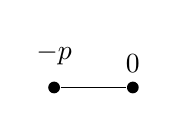
\begin{tikzpicture}[every node/.style={circle,fill=black,minimum width=1.5pt,inner sep=1.5pt}]
            \node[label={$-p$}] (A) at (0,0) {};
            \node[label={$0$}] (B) at (1,0) {};
            \draw (A) -- (B);
        \end{tikzpicture}
        \implies
        \begin{aligned}
            a_0 &= -1 & r_0 &= p \\
            a_1 &= 1 & r_1 &= 0
        \end{aligned}
    \end{equation*}
    Then, the action $\mathbb{T}^1 \acton \mathbb{C}^2$ is given by $\lambda \cdot (z_1, z_2) = (\lambda z_1, \lambda z_2)$. Also, we have the following data.
    \begin{equation*}
        \begin{tikzcd}[row sep=0ex]
            0 \arrow[r] & \mathfrak{t}^1 \arrow[r, "\iota"] & \mathfrak{t}^2 \arrow[r, "\pi"] & \mathfrak{t}^1 \arrow[r] & 0 \\
            {} & x \arrow[r, maps to] & (x, x) & {} & {} \\
            0 & (\mathfrak{t}^1)^* \arrow[l] & (\mathfrak{t}^2)^* \arrow[l, "\iota^*"'] & (\mathfrak{t}^1)^* \arrow[l, "\pi^*"'] & 0 \arrow[l] \\
            {} & x+y & (x, y) \arrow[l, maps to] & {} & {}
        \end{tikzcd}
    \end{equation*}
    Thus, the moment map $\iota^* \circ \mu : \mathbb{C}^2 \to (\mathfrak{t}^1)^*$ is given by
    \begin{equation*}
        \iota^*(\mu(z_1, z_2)) = \iota^*(-\pi|z_1|^2+p, -\pi|z_2|^2) = -\pi(|z_1|^2+|z_2|^2) + p.
    \end{equation*}
    Thus, $Z = (\iota^* \circ \mu)^{-1}(0) = \{ z \in \mathbb{C}^2 \mid |z|^2 = p/\pi \}$. Thinking $Z$ as $\mathbb{C}^2 / \mathbb{R}_{>0}$, $Z/\mathbb{T}^1 \cong \mathbb{P}^1$.
\end{example}

\begin{example}{}
    Consider the following polytope.
    \begin{equation*}
        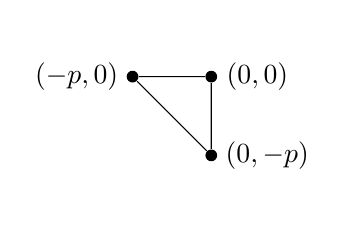
\begin{tikzpicture}[every node/.style={circle,fill=black,minimum width=1.5pt,inner sep=1.5pt}, baseline={(0,-0.5)}]
            \node[label={0:$(0,0)$}] (A) at (0,0) {};
            \node[label={180:$(-p,0)$}] (B) at (-1,0) {};
            \node[label={0:$(0,-p)$}] (C) at (0,-1) {};
            \draw (A) -- (B) -- (C) -- (A);
        \end{tikzpicture}
        \implies
        \begin{aligned}
            a_0 &= (-1,-1) & r_0 &= p \\
            a_1 &= (1,0) & r_1 &= 0 \\
            a_2 &= (0,1) & r_2 &= 0
        \end{aligned}
    \end{equation*}
    Then, the action $\mathbb{T} \acton \mathbb{C}^3$ is given by $\lambda \cdot (z_0, z_1, z_2) = (\lambda z_0, \lambda z_1, \lambda z_2)$. Also, we have the following data.
    \begin{equation*}
        \begin{tikzcd}[row sep=0ex]
            0 \arrow[r] & \mathfrak{t}^1 \arrow[r, "\iota"] & \mathfrak{t}^3 \arrow[r, "\pi"] & \mathfrak{t}^2 \arrow[r] & 0 \\
            {} & x \arrow[r, maps to] & (x, x, x) & {} & {} \\
            0 & (\mathfrak{t}^1)^* \arrow[l] & (\mathfrak{t}^3)^* \arrow[l, "\iota^*"'] & (\mathfrak{t}^2)^* \arrow[l, "\pi^*"'] & 0 \arrow[l] \\
            {} & x+y+z & (x, y, z) \arrow[l, maps to] & {} & {}
        \end{tikzcd}
    \end{equation*}
    Thus, the moment map $\iota^* \circ \mu : \mathbb{C}^3 \to (\mathfrak{t}^1)^*$ of is given by
    \begin{equation*}
        \iota^*(\mu(z_0, z_1, z_2)) = \iota^*(-\pi|z_0|^2, -\pi|z_1|^2, \pi|z_2|^2+p) = -\pi(|z_0|^2+|z_1|^2+|z_2|^2) + p.
    \end{equation*}
    Thus, $Z = (\iota^* \circ \mu)^{-1}(0) = \{ z \in \mathbb{C}^3 \mid |z|^2 = p/\pi \}$. Thinking $Z$ as $\mathbb{C}^3 / \mathbb{R}_{>0}$, $Z/\mathbb{T}^1 \cong \mathbb{P}^2$.
\end{example}

\begin{example}{}
    Denote the standard basis of $\mathbb{R}^n$ by $e_i$. Consider the following polytope.
    \begin{equation*}
        \mathrm{conv}(\{ 0, e_1, \dots, e_n \})
        \implies
        \begin{aligned}
            a_0 &= (-1, \dots, -1) & r_0 &= p \in \mathbb{Z}_{>0} \\
            a_i &= e_i & r_i &= 0 \quad \forall 1 \leq i \leq n
        \end{aligned}
    \end{equation*}
    Then, the action $\mathbb{T} \acton \mathbb{C}^{n+1}$ is given by $\lambda \cdot (z_0, \dots, z_n) = (\lambda z_0, \dots, \lambda z_n)$. Also, we have the following data.
    \begin{equation*}
        \begin{tikzcd}[row sep=0ex]
            0 \arrow[r] & \mathfrak{t}^1 \arrow[r, "\iota"] & \mathfrak{t}^{n+1} \arrow[r, "\pi"] & \mathfrak{t}^n \arrow[r] & 0 \\
            {} & x \arrow[r, maps to] & (x, \dots, x) & {} & {} \\
            0 & (\mathfrak{t}^1)^* \arrow[l] & (\mathfrak{t}^{n+1})^* \arrow[l, "\iota^*"'] & (\mathfrak{t}^n)^* \arrow[l, "\pi^*"'] & 0 \arrow[l] \\
            {} & x_0 + \cdots + x_n & (x_0, \dots, x_n) \arrow[l, maps to] & {} & {}
        \end{tikzcd}
    \end{equation*}
    Thus, the moment map $\iota^* \circ \mu : \mathbb{C}^3 \to (\mathfrak{t}^1)^*$ of is given by
    \begin{equation*}
        \iota^*(\mu(z_0, \dots, z_n)) = \iota^*(-\pi|z_0|^2+p, -\pi|z_1|^2, \dots, \pi|z_n|^2) = -\pi(|z_0|^2+\cdots+|z_n|^2) + p.
    \end{equation*}
    Thus, $Z = (\iota^* \circ \mu)^{-1}(0) = \{ z \in \mathbb{C}^{n+1} \mid |z|^2 = p/\pi \}$. Thinking $Z$ as $\mathbb{C}^{n+1} / \mathbb{R}_{>0}$, $Z/\mathbb{T}^1 \cong \mathbb{P}^n$.
\end{example}

\section{Lie Group and Lie Algebra}

\subsection{Vector Fields and Differential Forms}

\begin{notation}{} \strut
    \begin{enumerate}
        \item Smooth functions $M \to \mathbb{R}$: $\smth(M)$.
        \item Vector fields on $M$: $\vf(M)$.
        \item Differential $k$-forms on $M$: $\df^k(M)$.
    \end{enumerate}
\end{notation}

\begin{definition}{} \strut
    \begin{enumerate}
        \item Closed $k$-forms: $Z^k(M) = \ker(d : \df^k(M) \to \df^{k+1}(M))$.
        \item Exact $k$-forms: $B^k(M) = \im(d : \df^{k-1}(M) \to \df^k(M))$.
        \item $k$-th cohomology: $H^k(M) = Z^k(M)/B^k(M)$.
    \end{enumerate}
\end{definition}

\begin{notation}{} \strut
    \begin{enumerate}
        \item Exterior derivative: $d : \df^k(M) \to \df^{k+1}(M)$.
        \item Lie derivative: $\lied{X} : \df^k(M) \to \df^k(M)$ for all $X \in \vf(M)$.
        \item Interior derivative: $\intd{X} : \df^k(M) \to \df^{k-1}(M)$ for all $X \in \vf(M)$.
    \end{enumerate}
    \begin{remark}
    These give the following diagram.
        \begin{equation*}
            \begin{tikzcd}
                % {} & \smth(M) \arrow[d, equal] & {} & {} & {} \\
                0 \arrow[r, shift left, "!"] & \df^0(M) \arrow[loop above, "\lied{X}"] \arrow[r, shift left, "d"] \arrow[l, shift left, "!"] & \df^1(M) \arrow[loop above, "\lied{X}"] \arrow[r, shift left, "d"] \arrow[l, shift left, "\intd{X}"] & \df^2(M) \arrow[loop above, "\lied{X}"] \arrow[r, shift left, "d"] \arrow[l, shift left, "\intd{X}"] & \cdots \arrow[l, shift left, "\intd{X}"] \\[-1.5ex]
                & \smth(M) \arrow[u, equal]
            \end{tikzcd}
        \end{equation*}
\end{remark}
\end{notation}

\begin{lemma}[lem:prop_of_DLI]{Properties of $d$, $\lied{X}$, $\intd{X}$} \strut
    \begin{enumerate}
        \item $d^2 = 0$.
        \item $\lied{X} = d\intd{X} + \intd{X}d$.
        \item $\intd{[X, Y]} = \lied{X}\intd{Y} - \intd{Y}\lied{X}$.
        \item $\lied{X}d = d\lied{X}$.
    \end{enumerate}
\end{lemma}

\subsection{Lie Group and Lie Algebra}

Let $G$ be a Lie group and $\mathfrak{g}$ be the corresponding Lie algebra. Then, we have the canonical identification $\mathfrak{g} \cong T_eG$. Lie group and Lie algebra homomorphisms are related by the following.
\begin{definition}{Induced Lie Algebra Homomorphism}
    Given $\varphi : G \to H$, $\ind{\varphi} : \mathfrak{g} \to \mathfrak{h}$ defined by $\ind{\varphi} = d\varphi_e$, i.e. the differential of $\varphi$ at the identity of $G$.
\end{definition}

For each $g \in G$, consider the conjugation $C_g : G \to G$ given by $x \mapsto gxg^{-1}$. This induces representations of $G$ on $\mathfrak{g}$ and $\mathfrak{g}^*$ respectively.

\begin{definition}{Adjoint Action}
    $\mathrm{Ad} : G \to \mathrm{GL}(\mathfrak{g})$ defined by $\mathrm{Ad}_g(X) = \ind{C_g}(X)$.
\end{definition}

\begin{definition}[def:coadj]{Coadjoint Action}
    $G \acton \mathfrak{g}^*$ dual of the adjoint action.
\end{definition}

\subsection{Lie Group Action}

\begin{notation}{Set of Diffeomorphisms $M \to M$}
    $\Diff(M)$.
\end{notation}

\begin{definition}{Lie Group Action}
    Group homomorphism $\rho : G \to \Diff(M)$ such that the induced map $G \times M \to M$ is smooth.
    \begin{remark}
        We think of it as a `Lie group homomorphism' $\rho : G \to \Diff(M)$.
    \end{remark}
\end{definition}

\begin{definition}[def:ind_vf]{Induced Vector Field}
    $X \in \mathfrak{g}$ gives $\ind{X} \in \vf(M)$ define by
    \begin{equation*}
        \ind{X}_p = \frac{d}{dt}[\exp(tX) \cdot p]_{t=0}
    \end{equation*}
    for all $p \in M$. This defines a map $\mathfrak{g} \to \vf(M) : X \mapsto \ind{X}$.
    \begin{remark}
        The Lie algebra of the `Lie group' $\Diff(M)$ is $(\vf(M), -[-, -])$, and the induced Lie algebra homomorphism of $\rho$ is precisely the map $\mathfrak{g} \to \vf(M) : X \mapsto \ind{X}$.
    \end{remark}
\end{definition}

\begin{theorem}[thm:QMT]{Quotient Manifold Theorem}
    Let $G \acton M$ be a free and proper action. Then, $M/G$ is a smooth manifold and $M \to M/G$ is a principal $G$-bundle.
    \begin{remark}
        In particular, the properness of the action is satisfied when $G$ is compact.
    \end{remark}
\end{theorem}

By principal $G$-bundle, we mean the following:

\begin{definition}[def:]{Principle $G$-bundle}
  A \vocab{principle $G$-bundle} is a map of spaces:
\[
  \xymatrix{E\ar[d]^\pi\\B}
\]
where $E$ is a $G$-space and $\pi$ looks locally like the first projection $E'\times G\rightarrow E'$ (with the $G$-action trivial on $E'$).
\end{definition}

\subsubsection*{Example Calculation of Induced Vector Field}

\begin{example}[exp:Cn_ind_vf]{$\mathbb{T}^n \acton \mathbb{C}^n$}
    We aim to find a Lie algebra homomorphism $\mathfrak{t}^n \to \vf(\mathbb{C}^n)$. Let $X_i \in \mathfrak{t}^n$ be a standard basis vector. The exponential map is given by
    \begin{equation*}
        \exp(tX_i) = (1, \dots, 1, e^{2\pi it}, 1, \dots, 1) \text{ at the $i$th entry}.
    \end{equation*}
    Then, the induced vector field $\ind{X_i}$ is given by the following.
    \begin{align*}
        (\ind{X_i})_z &= \frac{d}{dt} [(z_1, \dots, e^{2\pi it} z_i, \dots, z_n)]_{t=0} \\
        &= \frac{d}{dt} [(x_1, \dots, \cos(2\pi t) x_i - \sin(2\pi t) y_i, \dots, x_n, y_1, \dots, \sin(2\pi t)x_i + \cos(2\pi t)y_i, \dots, y_n)]_{t=0} \\
        &= (0, \dots, -2\pi y_i, \dots, 0, 0, \dots, 2\pi x_i, \dots, 0) = -2\pi y_i \left.\frac{\partial}{\partial x_i}\right|_z + 2\pi x_i \left.\frac{\partial}{\partial y_i}\right|_z.
    \end{align*}
    Thus, we have $\ind{X_i} = -2\pi y_i \frac{\partial}{\partial x_i} + 2\pi x_i \frac{\partial}{\partial y_i}$.
    \begin{remark}
        Thinking $\mathfrak{t}^n$ as the tangent space of $\mathbb{T}^n$, $\exp(tX_i)$ is just the one parameter subgroup of $\mathbb{T}^n$ whose derivative at 0 is $X_i$.
    \end{remark}
    \begin{remark}
        The $2\pi$ in the equations are somehow just a convention, which comes down to the specific choice of isomorphism $\mathfrak{t}^n \cong \mathbb{R}^n$.
    \end{remark}
\end{example}

%\bibliographystyle{alpha}
%\bibliography{ref}

\end{document}
